\documentclass[12pt,a4paper]{article}

\usepackage[utf8]{inputenc}
\usepackage[T1]{fontenc}
\usepackage[brazil]{babel}
\usepackage{geometry}
\usepackage{graphicx}
\usepackage{float}
\usepackage{hyperref}
\usepackage{listings}
\usepackage{xcolor}
\usepackage{longtable}

\geometry{margin=2.5cm}

\lstdefinestyle{sqlstyle}{
    language=SQL,
    basicstyle=\ttfamily\small,
    keywordstyle=\color{blue},
    commentstyle=\color{gray},
    stringstyle=\color{red!60!black},
    breaklines=true,
    frame=single,
    columns=fullflexible
}

\title{
    \textbf{Projeto Final P4}\\
    Laboratorio de Bases de Dados\\
    Base Formula 1, Cidades e Aeroportos
}

\author{
    Nome 1 -- NUSP \\
    Nome 2 -- NUSP \\
    Nome 3 -- NUSP
}

\date{Junho de 2026}

\begin{document}

\maketitle

\section{Introducao}

Este trabalho apresenta o desenvolvimento de um prototipo de aplicacao completa para exploracao da base de dados da Formula 1 integrada a dados geograficos de cidades, paises e aeroportos.

A aplicacao permite autenticar usuarios com perfis distintos, apresentar dashboards personalizados, executar relatorios e realizar operacoes de cadastro conforme as permissoes de cada tipo de usuario.

\section{Preparacao da Base de Dados}

A base utilizada foi preparada a partir dos scripts desenvolvidos ao longo da disciplina. A execucao foi organizada na seguinte ordem:

\begin{enumerate}
    \item \texttt{create\_table.sql}: criacao do esquema relacional;
    \item \texttt{insert\_table.sql}: carga dos arquivos CSV e TSV;
    \item \texttt{clean\_data.sql}: normalizacao, deduplicacao e ajuste de vinculos;
    \item \texttt{app\_users.sql}: usuarios, autenticacao, auditoria e triggers;
    \item \texttt{app\_dashboard.sql}: funcoes de dashboard;
    \item \texttt{app\_reports.sql}: funcoes de relatorios;
    \item \texttt{app\_indexes.sql}: indices auxiliares.
\end{enumerate}

\subsection{Execucao com Docker}

Para facilitar a reproducao do ambiente entre os membros do grupo, foi utilizado Docker com PostgreSQL. O banco e carregado pelo script:

\begin{lstlisting}[style=sqlstyle]
./scripts/load_database.sh
\end{lstlisting}

Os dados de conexao utilizados foram:

\begin{itemize}
    \item Banco: \texttt{f1db}
    \item Usuario: \texttt{f1user}
    \item Porta: \texttt{5433}
\end{itemize}

\section{Modelo de Usuarios e Autenticacao}

A aplicacao possui tres tipos de usuario:

\begin{itemize}
    \item \textbf{Admin}: usuario administrador do sistema;
    \item \textbf{Escuderia}: usuario associado a uma escuderia;
    \item \textbf{Piloto}: usuario associado a um piloto.
\end{itemize}

Foi criada a tabela \texttt{users}, contendo os atributos \texttt{userid}, \texttt{login}, \texttt{password}, \texttt{tipo} e \texttt{id\_original}. O atributo \texttt{id\_original} referencia o identificador original de piloto ou escuderia, conforme o tipo de usuario.

\subsection{Protecao das Senhas}

A autenticacao foi implementada diretamente pela tabela \texttt{users}. Por isso, as senhas nao sao armazenadas em texto puro. Foi utilizada a extensao \texttt{pgcrypto}, com as funcoes \texttt{crypt()} e \texttt{gen\_salt()}.

\begin{lstlisting}[style=sqlstyle]
CREATE OR REPLACE FUNCTION app_hash_password(p_plain_password TEXT)
RETURNS TEXT AS $$
BEGIN
    RETURN crypt(p_plain_password, gen_salt('bf'));
END;
$$ LANGUAGE plpgsql;
\end{lstlisting}

\subsection{Auditoria de Acesso}

Foi criada a tabela \texttt{users\_log}, responsavel por registrar eventos de \texttt{LOGIN} e \texttt{LOGOUT}. A funcao \texttt{app\_login} registra automaticamente a entrada do usuario quando a autenticacao e realizada com sucesso.

\section{Triggers Implementadas}

\subsection{Sincronizacao de Pilotos com Usuarios}

A trigger associada a tabela \texttt{drivers} cria automaticamente um usuario do tipo \texttt{Piloto} sempre que um novo piloto e cadastrado.

\subsection{Sincronizacao de Escuderias com Usuarios}

A trigger associada a tabela \texttt{constructors} cria automaticamente um usuario do tipo \texttt{Escuderia} sempre que uma nova escuderia e cadastrada.

\subsection{Atualizacao de Data em Usuarios}

A trigger de atualizacao da tabela \texttt{users} atualiza automaticamente o campo \texttt{updated\_at} quando uma tupla e modificada.

\section{Dashboards}

\subsection{Dashboard do Administrador}

O dashboard do administrador apresenta:

\begin{itemize}
    \item quantidade total de pilotos, escuderias e temporadas;
    \item corridas cadastradas na temporada mais recente;
    \item escuderias da temporada mais recente com total de pontos;
    \item pilotos da temporada mais recente com total de pontos.
\end{itemize}

\subsection{Dashboard da Escuderia}

O dashboard da escuderia apresenta:

\begin{itemize}
    \item quantidade de vitorias da escuderia;
    \item quantidade de pilotos diferentes que ja correram pela escuderia;
    \item primeiro e ultimo ano com dados da escuderia.
\end{itemize}

\subsection{Dashboard do Piloto}

O dashboard do piloto apresenta:

\begin{itemize}
    \item primeiro e ultimo ano com dados do piloto;
    \item desempenho por ano e circuito, incluindo pontos, vitorias e corridas disputadas.
\end{itemize}

\section{Relatorios}

\subsection{Relatorio 1 -- Admin: Resultados por Status}

Este relatorio apresenta a quantidade de resultados agrupados por status de corrida.

\subsection{Relatorio 2 -- Admin: Aeroportos Proximos a Cidade Brasileira}

Este relatorio recebe o nome de uma cidade e retorna aeroportos brasileiros dos tipos \texttt{medium\_airport} e \texttt{large\_airport} localizados a ate 100 km da cidade pesquisada.

Para o calculo de distancia foi utilizada a extensao \texttt{earthdistance}, juntamente com \texttt{cube}.

\begin{lstlisting}[style=sqlstyle]
earth_distance(
    ll_to_earth(c.latitude, c.longitude),
    ll_to_earth(a.latitude_deg, a.longitude_deg)
) / 1000.0
\end{lstlisting}

\subsection{Relatorio 3 -- Admin: Relatorio Hierarquico de Corridas}

O relatorio hierarquico foi organizado em tres niveis:

\begin{enumerate}
    \item total de corridas cadastradas;
    \item estatisticas de corridas por circuito;
    \item detalhes das corridas de cada circuito.
\end{enumerate}

\subsection{Relatorio 4 -- Escuderia: Vitorias por Piloto}

Este relatorio lista os pilotos que correram por uma escuderia e a quantidade de vezes em que cada piloto obteve primeira posicao.

\subsection{Relatorio 5 -- Escuderia: Resultados por Status}

Este relatorio apresenta a quantidade de resultados por status, limitada ao escopo da escuderia logada.

\subsection{Relatorio 6 -- Piloto: Pontos por Ano e Corridas}

Este relatorio apresenta os pontos obtidos pelo piloto por ano de participacao, indicando as corridas em que os pontos foram obtidos.

\subsection{Relatorio 7 -- Piloto: Status das Corridas}

Este relatorio apresenta a quantidade de resultados por status nas corridas em que o piloto participou.

\section{Indices Criados}

Os indices foram criados para auxiliar consultas com filtros, juncoes e ordenacoes frequentes.

\begin{longtable}{|p{5cm}|p{8cm}|}
\hline
\textbf{Indice} & \textbf{Justificativa} \\
\hline
\texttt{results(driver\_id)} & Auxilia dashboards e relatorios de pilotos. \\
\hline
\texttt{results(constructor\_id)} & Auxilia dashboards e relatorios de escuderias. \\
\hline
\texttt{results(status\_id)} & Auxilia relatorios de contagem por status. \\
\hline
\texttt{races(season\_id)} & Auxilia consultas por temporada. \\
\hline
\texttt{races(circuit\_id)} & Auxilia relatorio hierarquico por circuito. \\
\hline
\texttt{cities(country\_id, name)} & Auxilia busca de cidades brasileiras por nome. \\
\hline
\end{longtable}

\section{Interface da Aplicacao}

A interface foi organizada em tres telas principais:

\begin{itemize}
    \item tela de login;
    \item tela de dashboard;
    \item tela de relatorios.
\end{itemize}

\subsection{Tela de Login}

Inserir descricao e captura de tela.

\begin{figure}[H]
    \centering
    % 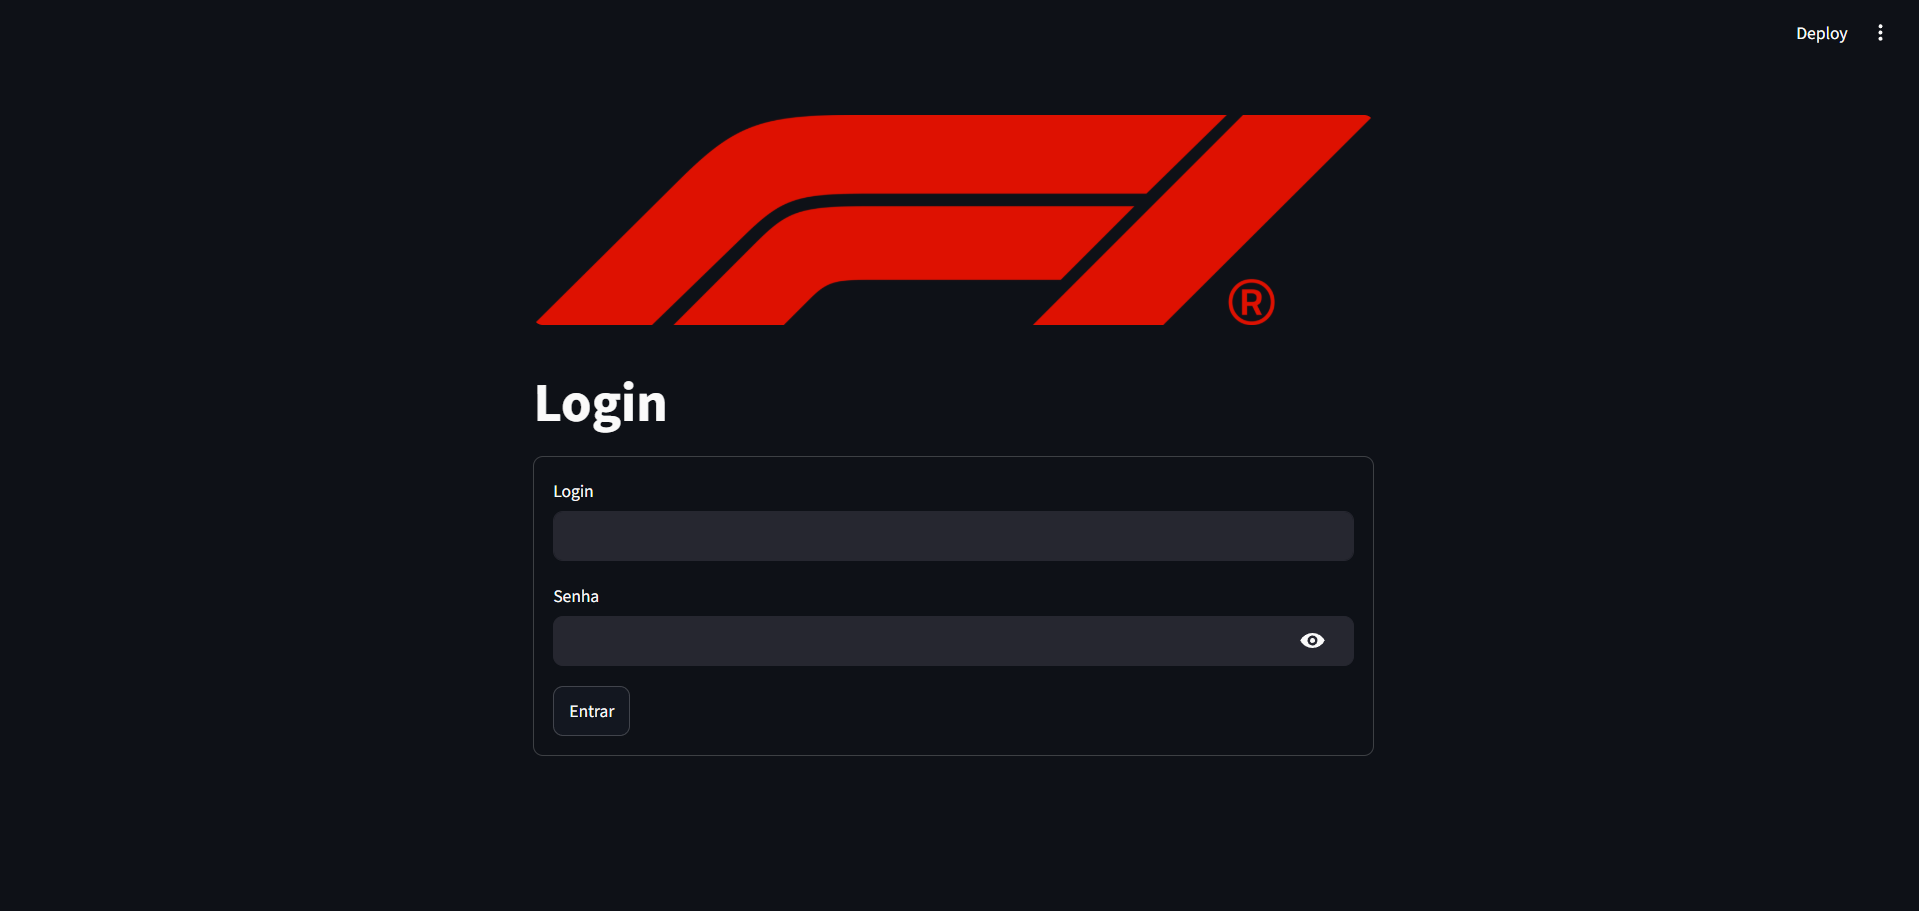
\includegraphics[width=0.85\textwidth]{screenshots/login.png}
    \caption{Tela de login da aplicacao.}
\end{figure}

\subsection{Tela de Dashboard}

Inserir descricao e captura de tela.

\begin{figure}[H]
    \centering
    % 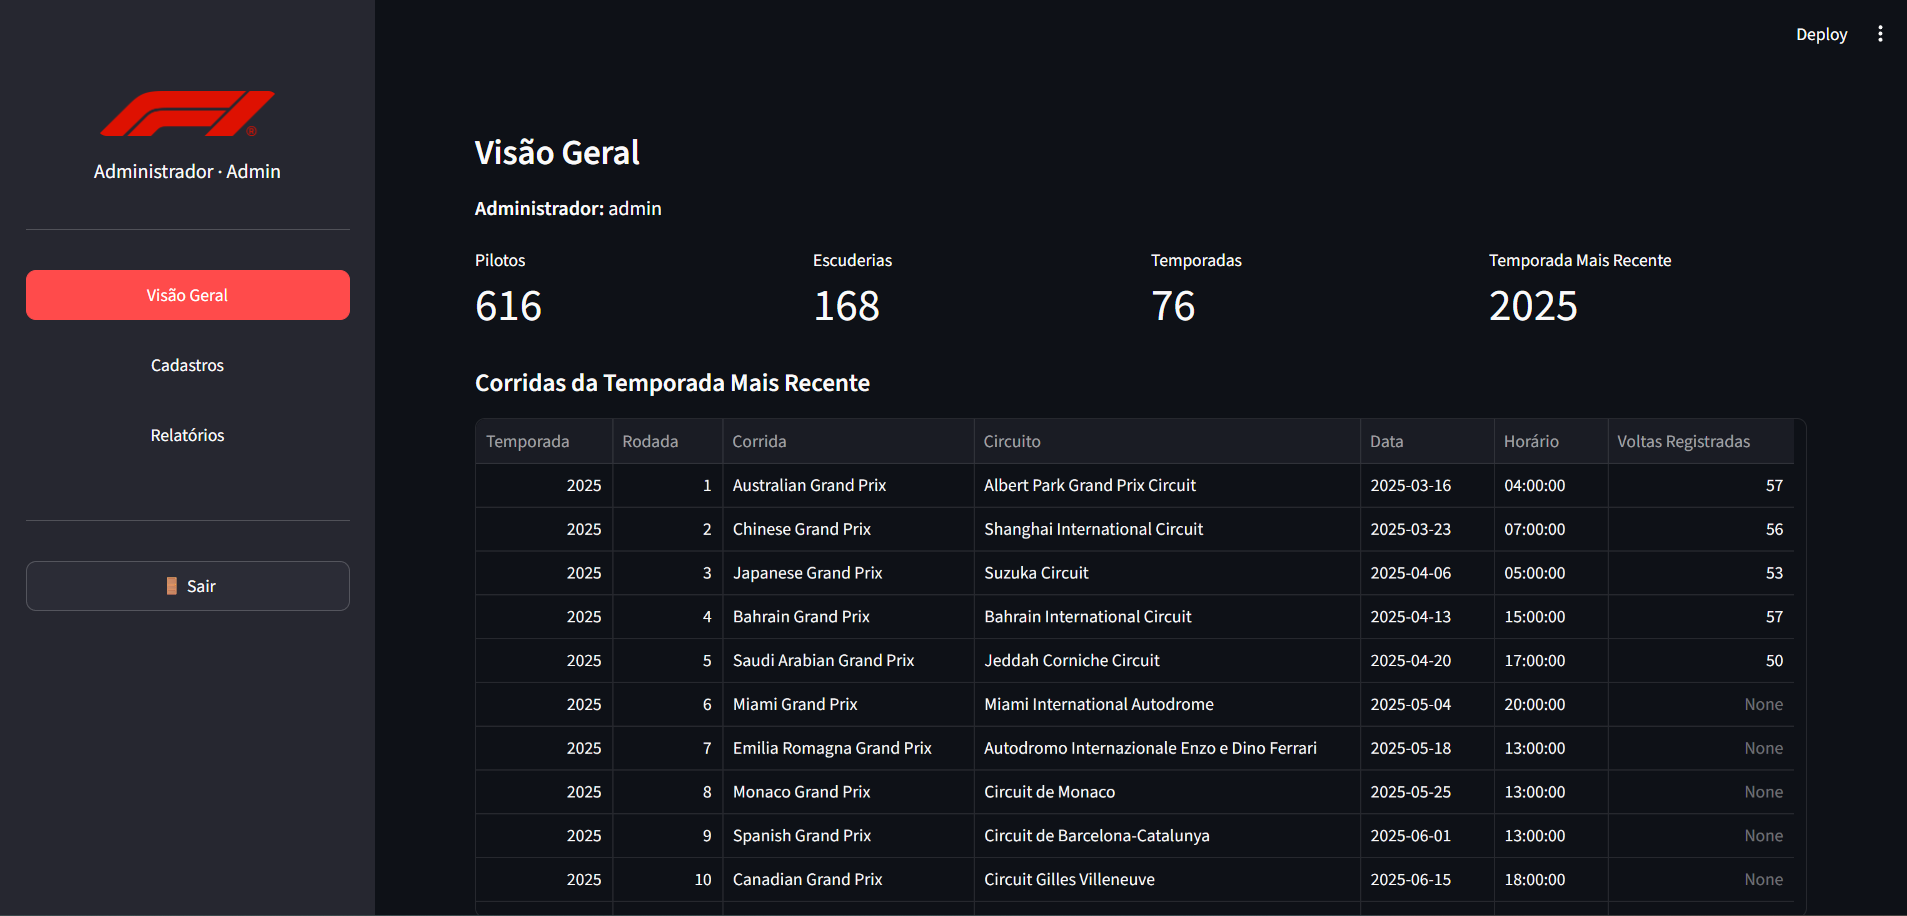
\includegraphics[width=0.85\textwidth]{screenshots/dashboard.png}
    \caption{Tela de dashboard.}
\end{figure}

\subsection{Tela de Relatorios}

Inserir descricao e captura de tela.

\begin{figure}[H]
    \centering
    % 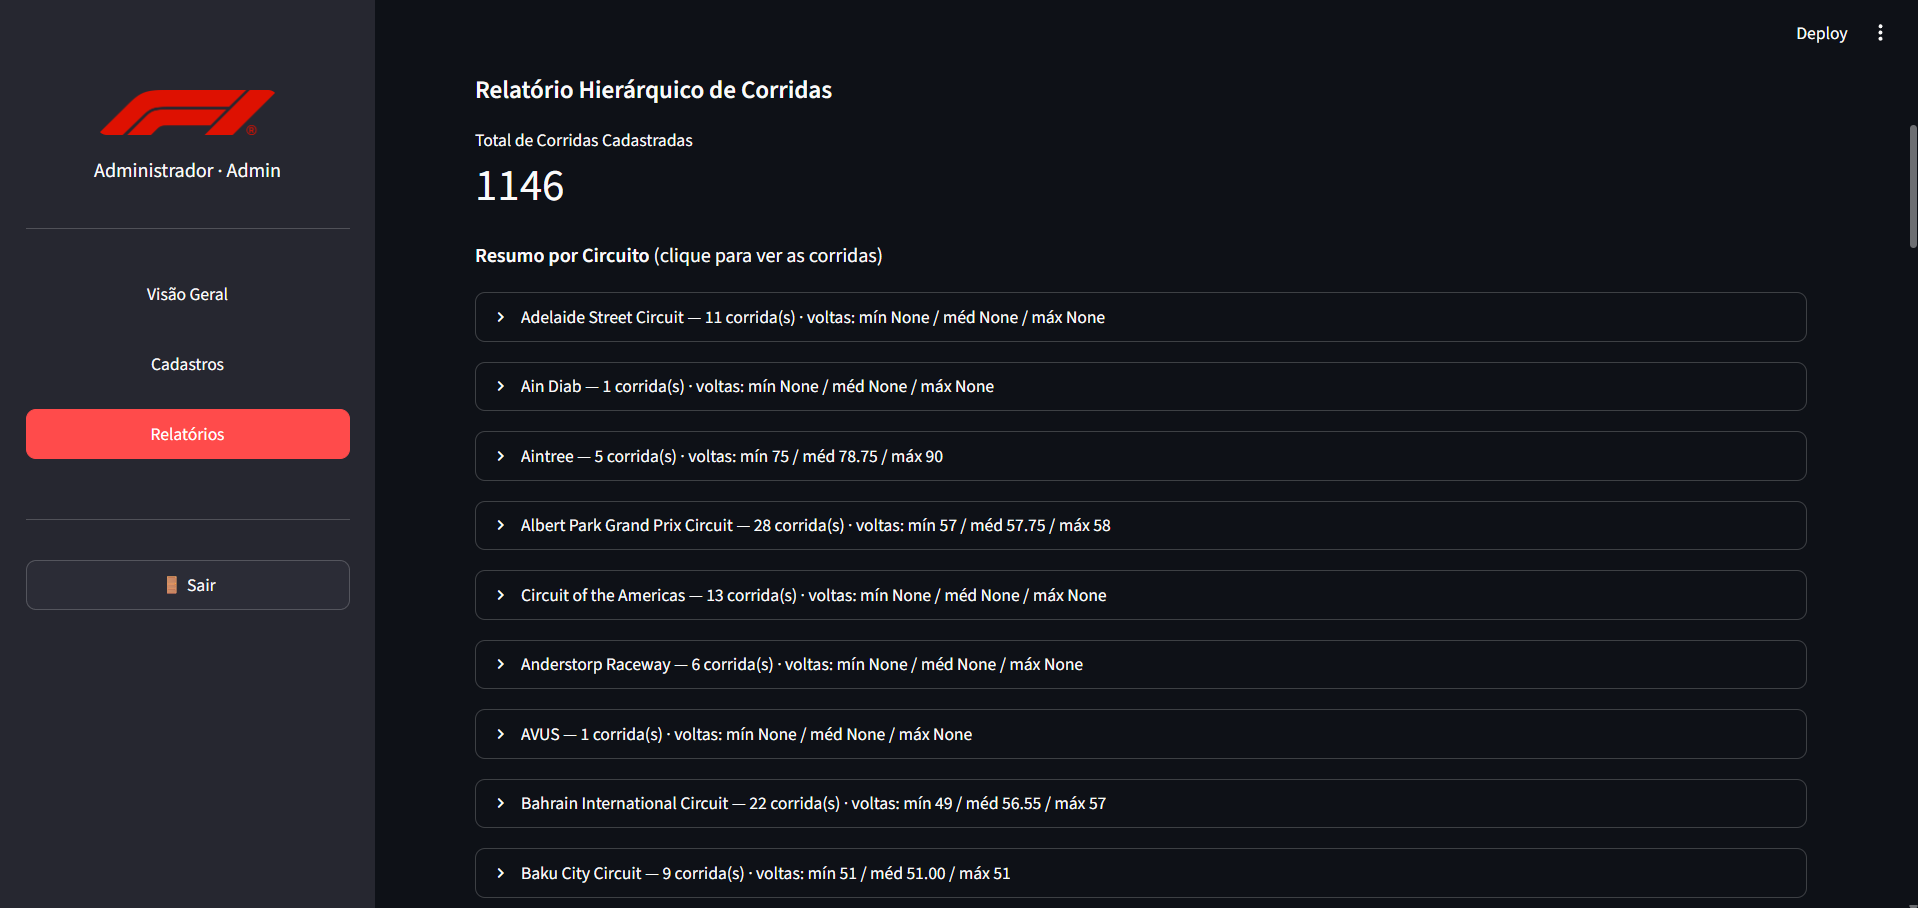
\includegraphics[width=0.85\textwidth]{screenshots/relatorios.png}
    \caption{Tela de relatorios.}
\end{figure}

\section{Decisoes de Projeto}

\begin{itemize}
    \item A autenticacao foi feita pela tabela \texttt{users}, e nao por usuarios reais do PostgreSQL, para simplificar a integracao com a aplicacao.
    \item As senhas foram armazenadas com hash usando \texttt{pgcrypto}.
    \item O ambiente de execucao foi containerizado com Docker para facilitar a reproducao.
    \item Os relatorios e dashboards foram implementados como funcoes armazenadas, mantendo os comandos SQL explicitos.
\end{itemize}

\section{Dificuldades Encontradas}

Descrever aqui as principais dificuldades, por exemplo:

\begin{itemize}
    \item compatibilizacao entre os nomes dos arquivos CSV e o esquema relacional;
    \item normalizacao de nacionalidades;
    \item deduplicacao de cidades;
    \item calculo de distancia entre coordenadas geograficas;
    \item organizacao dos diferentes tipos de usuario.
\end{itemize}

\section{Conclusao}

O projeto integrou os conceitos estudados na disciplina por meio da construcao de uma aplicacao apoiada por banco de dados relacional, utilizando carga e limpeza de dados, funcoes, triggers, indices, autenticacao, auditoria, dashboards e relatorios.

\end{document}
